% Options for packages loaded elsewhere
\PassOptionsToPackage{unicode}{hyperref}
\PassOptionsToPackage{hyphens}{url}
%
\documentclass[
  ignorenonframetext,
]{beamer}
\usepackage{pgfpages}
\setbeamertemplate{caption}[numbered]
\setbeamertemplate{caption label separator}{: }
\setbeamercolor{caption name}{fg=normal text.fg}
\beamertemplatenavigationsymbolsempty
% Prevent slide breaks in the middle of a paragraph
\widowpenalties 1 10000
\raggedbottom
\setbeamertemplate{part page}{
  \centering
  \begin{beamercolorbox}[sep=16pt,center]{part title}
    \usebeamerfont{part title}\insertpart\par
  \end{beamercolorbox}
}
\setbeamertemplate{section page}{
  \centering
  \begin{beamercolorbox}[sep=12pt,center]{part title}
    \usebeamerfont{section title}\insertsection\par
  \end{beamercolorbox}
}
\setbeamertemplate{subsection page}{
  \centering
  \begin{beamercolorbox}[sep=8pt,center]{part title}
    \usebeamerfont{subsection title}\insertsubsection\par
  \end{beamercolorbox}
}
\AtBeginPart{
  \frame{\partpage}
}
\AtBeginSection{
  \ifbibliography
  \else
    \frame{\sectionpage}
  \fi
}
\AtBeginSubsection{
  \frame{\subsectionpage}
}
\usepackage{amsmath,amssymb}
\usepackage{lmodern}
\usepackage{ifxetex,ifluatex}
\ifnum 0\ifxetex 1\fi\ifluatex 1\fi=0 % if pdftex
  \usepackage[T1]{fontenc}
  \usepackage[utf8]{inputenc}
  \usepackage{textcomp} % provide euro and other symbols
\else % if luatex or xetex
  \usepackage{unicode-math}
  \defaultfontfeatures{Scale=MatchLowercase}
  \defaultfontfeatures[\rmfamily]{Ligatures=TeX,Scale=1}
  \setmainfont[BoldFont = SF Pro Rounded Semibold]{SF Pro Rounded}
  \setmathfont[]{STIX Two Math}
\fi
\usefonttheme{serif} % use mainfont rather than sansfont for slide text
% Use upquote if available, for straight quotes in verbatim environments
\IfFileExists{upquote.sty}{\usepackage{upquote}}{}
\IfFileExists{microtype.sty}{% use microtype if available
  \usepackage[]{microtype}
  \UseMicrotypeSet[protrusion]{basicmath} % disable protrusion for tt fonts
}{}
\makeatletter
\@ifundefined{KOMAClassName}{% if non-KOMA class
  \IfFileExists{parskip.sty}{%
    \usepackage{parskip}
  }{% else
    \setlength{\parindent}{0pt}
    \setlength{\parskip}{6pt plus 2pt minus 1pt}}
}{% if KOMA class
  \KOMAoptions{parskip=half}}
\makeatother
\usepackage{xcolor}
\IfFileExists{xurl.sty}{\usepackage{xurl}}{} % add URL line breaks if available
\IfFileExists{bookmark.sty}{\usepackage{bookmark}}{\usepackage{hyperref}}
\hypersetup{
  pdftitle={305 Lecture 5.4 - Strategies 1: Working Backwards},
  pdfauthor={Brian Weatherson},
  hidelinks,
  pdfcreator={LaTeX via pandoc}}
\urlstyle{same} % disable monospaced font for URLs
\newif\ifbibliography
\usepackage{graphicx}
\makeatletter
\def\maxwidth{\ifdim\Gin@nat@width>\linewidth\linewidth\else\Gin@nat@width\fi}
\def\maxheight{\ifdim\Gin@nat@height>\textheight\textheight\else\Gin@nat@height\fi}
\makeatother
% Scale images if necessary, so that they will not overflow the page
% margins by default, and it is still possible to overwrite the defaults
% using explicit options in \includegraphics[width, height, ...]{}
\setkeys{Gin}{width=\maxwidth,height=\maxheight,keepaspectratio}
% Set default figure placement to htbp
\makeatletter
\def\fps@figure{htbp}
\makeatother
\setlength{\emergencystretch}{3em} % prevent overfull lines
\providecommand{\tightlist}{%
  \setlength{\itemsep}{0pt}\setlength{\parskip}{0pt}}
\setcounter{secnumdepth}{-\maxdimen} % remove section numbering
\let\Tiny=\tiny

 \setbeamertemplate{navigation symbols}{} 

% \usetheme{Madrid}
 \usetheme[numbering=none, progressbar=foot]{metropolis}
 \usecolortheme{wolverine}
 \usepackage{color}
 \usepackage{MnSymbol}
% \usepackage{movie15}

\usepackage{amssymb}% http://ctan.org/pkg/amssymb
\usepackage{pifont}% http://ctan.org/pkg/pifont
\newcommand{\cmark}{\ding{51}}%
\newcommand{\xmark}{\ding{55}}%

\DeclareSymbolFont{symbolsC}{U}{txsyc}{m}{n}
\DeclareMathSymbol{\boxright}{\mathrel}{symbolsC}{128}
\DeclareMathAlphabet{\mathpzc}{OT1}{pzc}{m}{it}

\usepackage{tikz-qtree}
% \usepackage{markdown}
%\RequirePackage{bussproofs}
\usetikzlibrary{arrows.meta}
\RequirePackage[tableaux]{prooftrees}
\forestset{line numbering, close with = x}
% Allow for easy commas inside trees
\renewcommand{\,}{\text{, }}


\usepackage{tabulary}

\usepackage{open-logic-config}

\setlength{\parskip}{1ex plus 0.5ex minus 0.2ex}

\AtBeginSection[]
{
\begin{frame}
	\Huge{\color{darkblue} \insertsection}
\end{frame}
}

\renewenvironment*{quote}	
	{\list{}{\rightmargin   \leftmargin} \item } 	
	{\endlist }

\definecolor{darkgreen}{rgb}{0,0.7,0}
\definecolor{darkblue}{rgb}{0,0,0.8}

\newcommand{\starttab}{\begin{center}
\vspace{6pt}
\begin{tabular}}

\newcommand{\stoptab}{\end{tabular}
\vspace{6pt}
\end{center}
\noindent}


\newcommand{\sif}{\rightarrow}
\newcommand{\siff}{\leftrightarrow}
\newcommand{\EF}{\end{frame}}


\newcommand{\TreeStart}[1]{
%\end{frame}
\begin{frame}
\begin{center}
\begin{tikzpicture}[scale=#1]
\tikzset{every tree node/.style={align=center,anchor=north}}
%\Tree
}

\newcommand{\TreeEnd}{
\end{tikzpicture}
%\end{center}
}

\newcommand{\DisplayArg}[2]{
\begin{enumerate}
{#1}
\end{enumerate}
\vspace{-6pt}
\hrulefill

%\hspace{14pt} #2
%{\addtolength{\leftskip}{14pt} #2}
\begin{quote}
{\normalfont #2}
\end{quote}
\vspace{12pt}
}

\newenvironment{ProofTree}[1][1]{
\begin{center}
\begin{tikzpicture}[scale=#1]
\tikzset{every tree node/.style={align=center,anchor=south}}
}
{
\end{tikzpicture}
\end{center}
}

\newcommand{\TreeFrame}[2]{
\begin{columns}[c]
\column{0.5\textwidth}
\begin{center}
\begin{prooftree}{}
#1
\end{prooftree}
\end{center}
\column{0.45\textwidth}
%\begin{markdown}
#2
%\end{markdown}
\end{columns}
}

\newcommand{\ScaledTreeFrame}[3]{
\begin{columns}[c]
\column{0.5\textwidth}
\begin{center}
\scalebox{#1}{
\begin{prooftree}{}
#2
\end{prooftree}
}
\end{center}
\column{0.45\textwidth}
%\begin{markdown}
#3
%\end{markdown}
\end{columns}
}

\usepackage[bb=boondox]{mathalfa}
\DeclareMathAlphabet{\mathbx}{U}{BOONDOX-ds}{m}{n}
\SetMathAlphabet{\mathbx}{bold}{U}{BOONDOX-ds}{b}{n}
\DeclareMathAlphabet{\mathbbx} {U}{BOONDOX-ds}{b}{n}


\newenvironment{oltableau}{\center\tableau{}} %wff format={anchor = base west}}}
       {\endtableau\endcenter}
       
\newcommand{\formula}[1]{$#1$}

\usepackage{tabulary}
\usepackage{booktabs}

\def\begincols{\begin{columns}}
\def\begincol{\begin{column}}
\def\endcol{\end{column}}
\def\endcols{\end{columns}}

\usepackage[italic]{mathastext}
\usepackage{nicefrac}

\definecolor{mygreen}{RGB}{0, 100, 0}
\definecolor{mypink2}{RGB}{219, 48, 122}
\definecolor{dodgerblue}{RGB}{30,144,255}

%\def\True{\textcolor{dodgerblue}{\text{T}}}
%\def\False{\textcolor{red}{\text{F}}}

\def\True{\mathbb{T}}
\def\False{\mathbb{F}}

% This is because arguments didn't have enough space after them
\usepackage{etoolbox}
\AfterEndEnvironment{description}{\vspace{9pt}}
\AfterEndEnvironment{oltableau}{\vspace{9pt}}
\BeforeBeginEnvironment{oltableau}{\vspace{9pt}}
\AfterEndEnvironment{center}{\vspace{12pt}}
\BeforeBeginEnvironment{tabular}{\vspace{9pt}}

\setlength\heavyrulewidth{0pt}
\setlength\lightrulewidth{0pt}

%\def\toprule{}
%\def\bottomrule{}
%\def\midrule{}

\setbeamertemplate{caption}{\raggedright\insertcaption}

\ifluatex
  \usepackage{selnolig}  % disable illegal ligatures
\fi

\title{305 Lecture 5.4 - Strategies 1: Working Backwards}
\author{Brian Weatherson}
\date{}

\begin{document}
\frame{\titlepage}

\begin{frame}{Plan}
\protect\hypertarget{plan}{}
This lecture discusses strategies for constructing proofs that involve
working backwards.
\end{frame}

\begin{frame}{Associated Reading}
\protect\hypertarget{associated-reading}{}
forall x, section 17.1.
\end{frame}

\begin{frame}{Big Picture}
\protect\hypertarget{big-picture}{}
\begin{itemize}
\tightlist
\item
  When you are given a proof to do, you are told what the intended
  conclusion is.
\item
  That conclusion will usually have a connective in it.
\item
  And when it does, it will often be good to aim to use the introduction
  rule for that connective to complete the proof.
\item
  Thinking about how that could happen will often give us something to
  aim for.
\end{itemize}
\end{frame}

\begin{frame}{Iteration}
\protect\hypertarget{iteration}{}
\begin{itemize}
\tightlist
\item
  The strategies they discuss in chapter 17 apply recursively.
\item
  Whenever we talk about a `target' or a `conclusion', that could be the
  conclusion of the whole argument, but it does not have to be.
\item
  It could just be something else we've set as a target.
\end{itemize}
\end{frame}

\begin{frame}{Working Backwards: And}
\protect\hypertarget{working-backwards-and}{}
The \(\wedge\)I rule says

\begin{itemize}
\tightlist
\item
  From X, and Y, infer X \(\wedge\) Y.
\end{itemize}

So if the last line is a conjunction, one strategy is to aim to prove
both parts.
\end{frame}

\begin{frame}{\(A \wedge B, C \vdash (A \wedge C) \wedge (B \wedge C)\)}
\protect\hypertarget{a-wedge-b-c-vdash-a-wedge-c-wedge-b-wedge-c}{}
\begin{figure}
\centering
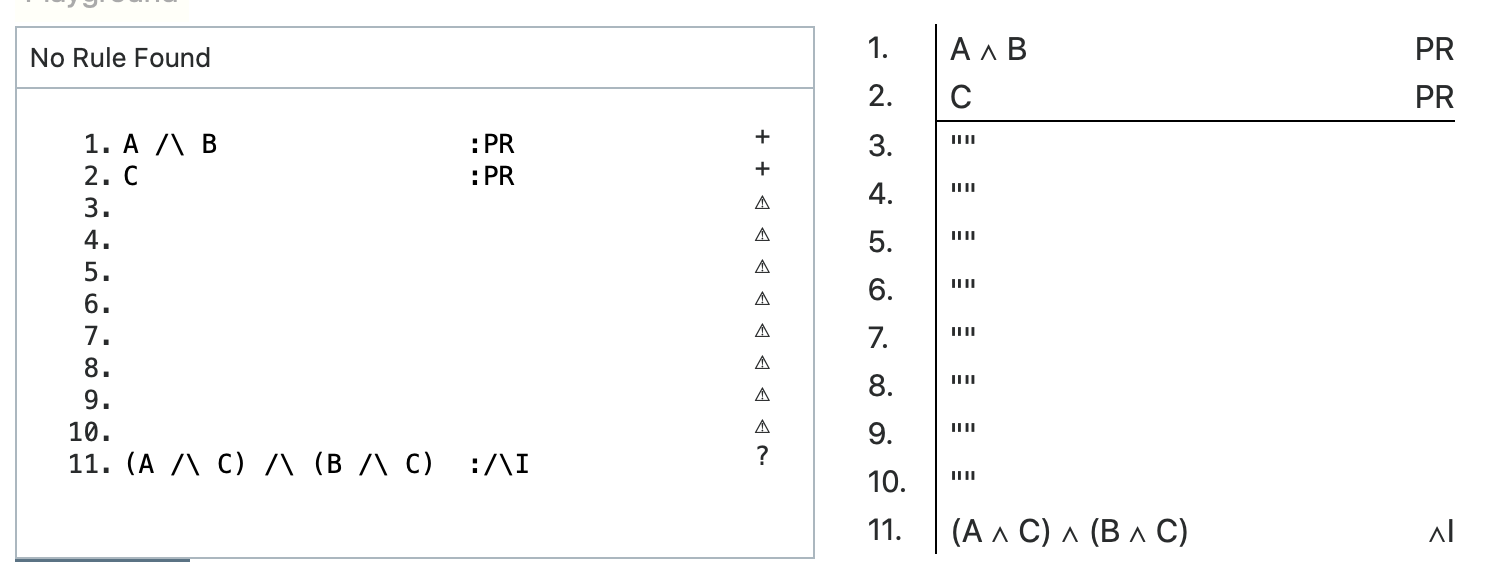
\includegraphics[width=\textwidth,height=0.75\textheight]{5_4a.png}
\caption{Writing out premises and conclusion}
\end{figure}
\end{frame}

\begin{frame}{\(A \wedge B, C \vdash (A \wedge C) \wedge (B \wedge C)\)}
\protect\hypertarget{a-wedge-b-c-vdash-a-wedge-c-wedge-b-wedge-c-1}{}
\begin{figure}
\centering
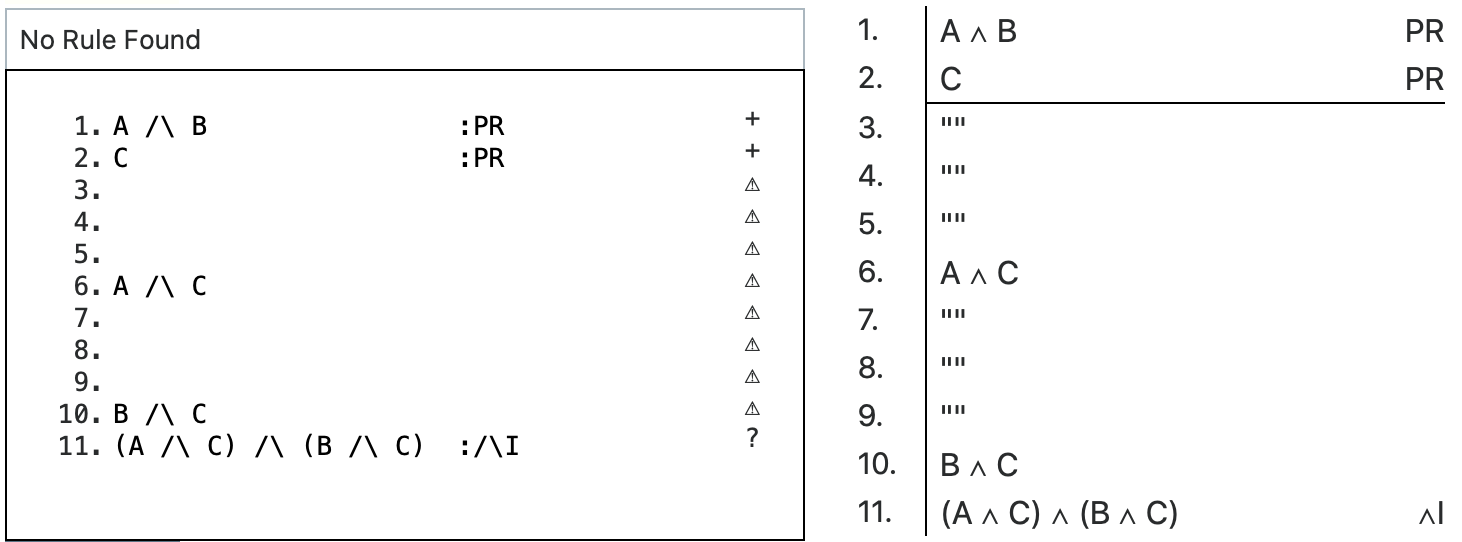
\includegraphics[width=\textwidth,height=0.75\textheight]{5_4b.png}
\caption{Setting up \(\wedge\) introduction}
\end{figure}
\end{frame}

\begin{frame}{\(A \wedge B, C \vdash (A \wedge C) \wedge (B \wedge C)\)}
\protect\hypertarget{a-wedge-b-c-vdash-a-wedge-c-wedge-b-wedge-c-2}{}
\begin{figure}
\centering
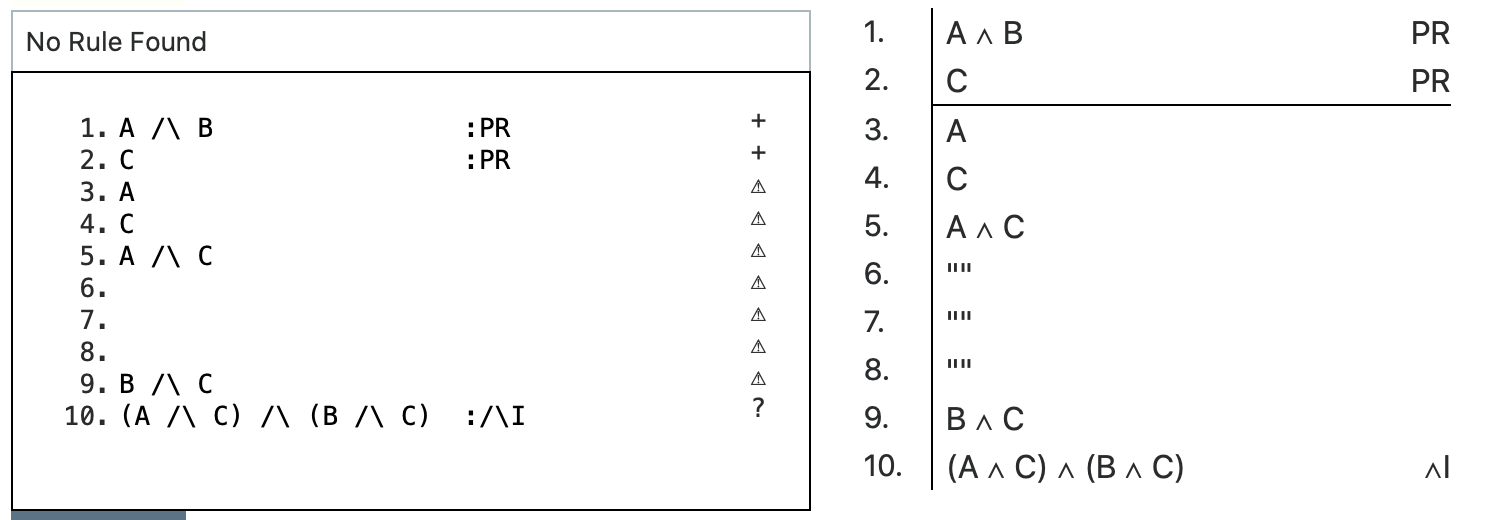
\includegraphics[width=\textwidth,height=0.75\textheight]{5_4c.png}
\caption{Working backwards from \(A \wedge C\)}
\end{figure}
\end{frame}

\begin{frame}{\(A \wedge B, C \vdash (A \wedge C) \wedge (B \wedge C)\)}
\protect\hypertarget{a-wedge-b-c-vdash-a-wedge-c-wedge-b-wedge-c-3}{}
\begin{figure}
\centering
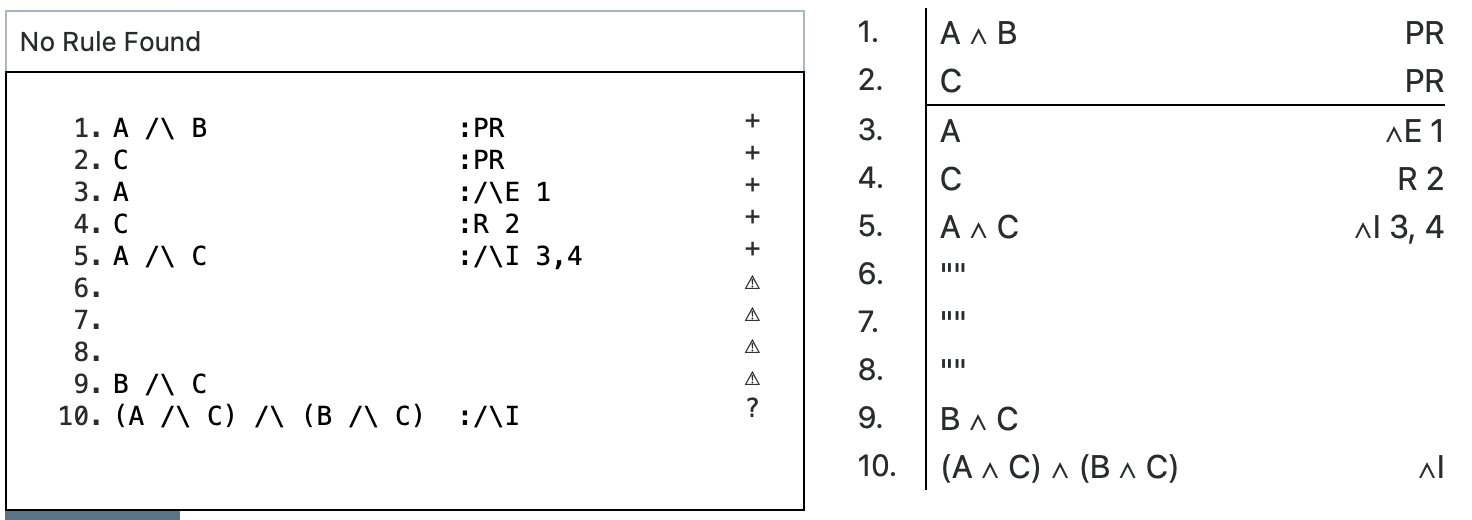
\includegraphics[width=\textwidth,height=0.75\textheight]{5_4d.png}
\caption{Filling in rules}
\end{figure}
\end{frame}

\begin{frame}{\(A \wedge B, C \vdash (A \wedge C) \wedge (B \wedge C)\)}
\protect\hypertarget{a-wedge-b-c-vdash-a-wedge-c-wedge-b-wedge-c-4}{}
\begin{figure}
\centering
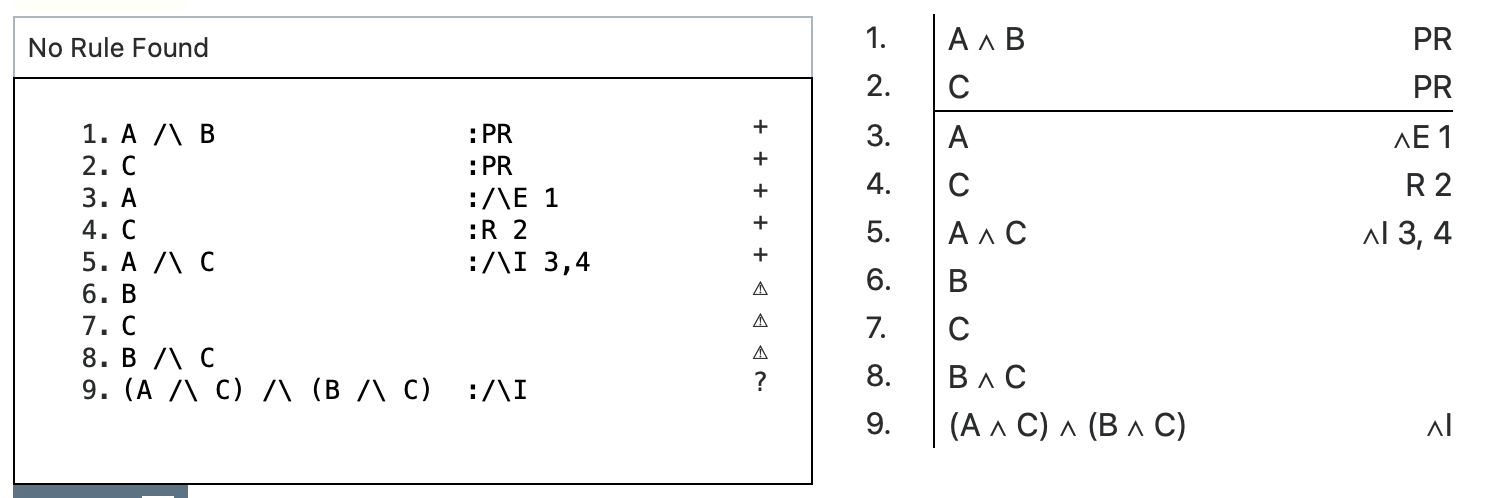
\includegraphics[width=\textwidth,height=0.75\textheight]{5_4e.png}
\caption{Working backwards from \(B \wedge C\)}
\end{figure}
\end{frame}

\begin{frame}{\(A \wedge B, C \vdash (A \wedge C) \wedge (B \wedge C)\)}
\protect\hypertarget{a-wedge-b-c-vdash-a-wedge-c-wedge-b-wedge-c-5}{}
\begin{figure}
\centering
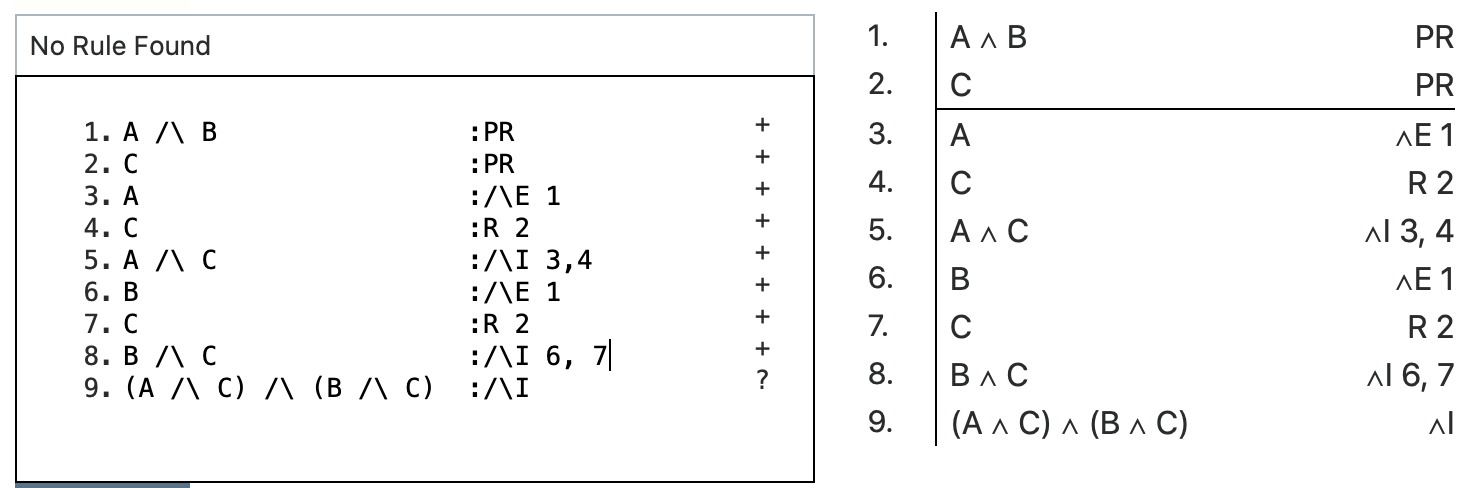
\includegraphics[width=\textwidth,height=0.75\textheight]{5_4f.png}
\caption{Filling in line numbers for the second half}
\end{figure}
\end{frame}

\begin{frame}{\(A \wedge B, C \vdash (A \wedge C) \wedge (B \wedge C)\)}
\protect\hypertarget{a-wedge-b-c-vdash-a-wedge-c-wedge-b-wedge-c-6}{}
\begin{figure}
\centering
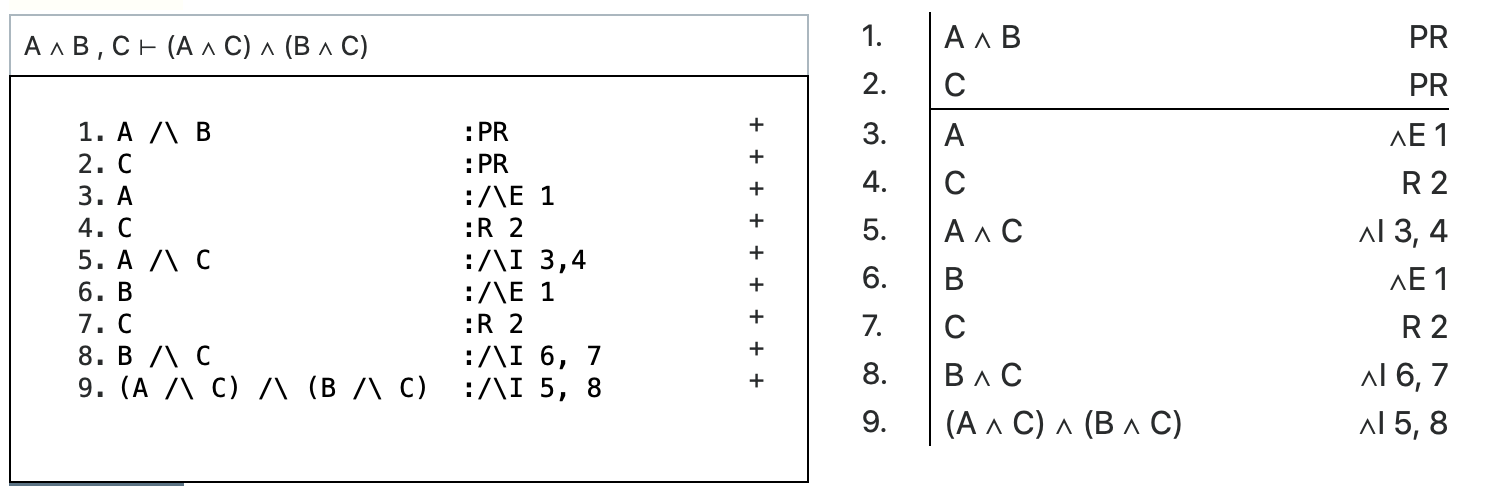
\includegraphics[width=\textwidth,height=0.75\textheight]{5_4g.png}
\caption{Filling in line numbers for the final line}
\end{figure}
\end{frame}

\begin{frame}{\(A \rightarrow B \vdash (A \wedge C) \rightarrow (B \wedge C)\)}
\protect\hypertarget{a-rightarrow-b-vdash-a-wedge-c-rightarrow-b-wedge-c}{}
\begin{figure}
\centering
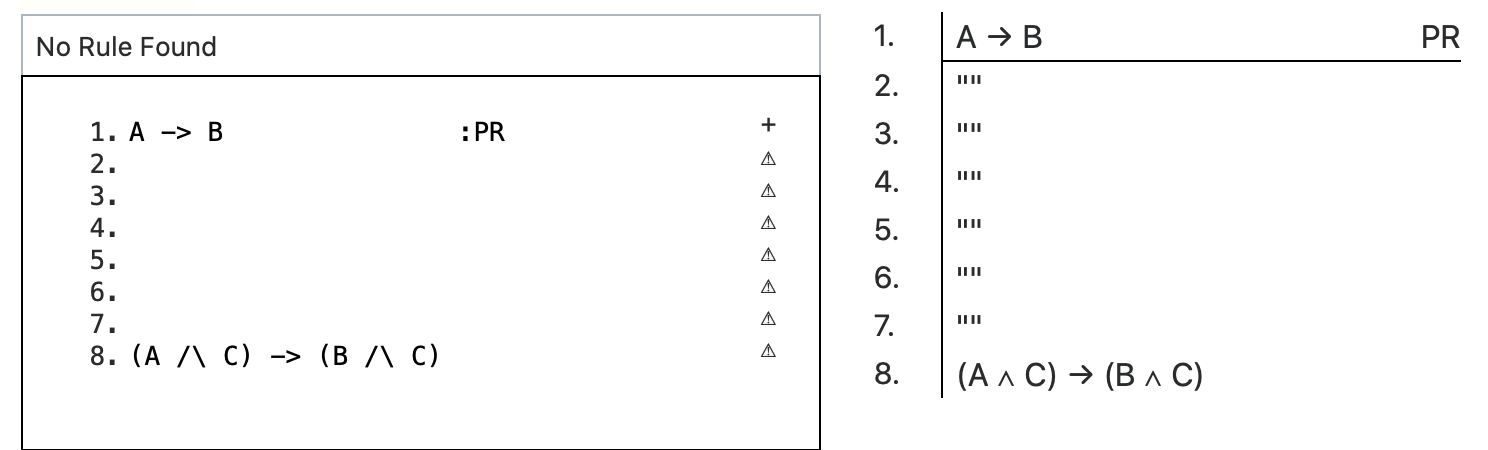
\includegraphics[width=\textwidth,height=0.75\textheight]{5_4h.png}
\caption{Premise and conclusion}
\end{figure}
\end{frame}

\begin{frame}{\(A \rightarrow B \vdash (A \wedge C) \rightarrow (B \wedge C)\)}
\protect\hypertarget{a-rightarrow-b-vdash-a-wedge-c-rightarrow-b-wedge-c-1}{}
\begin{figure}
\centering
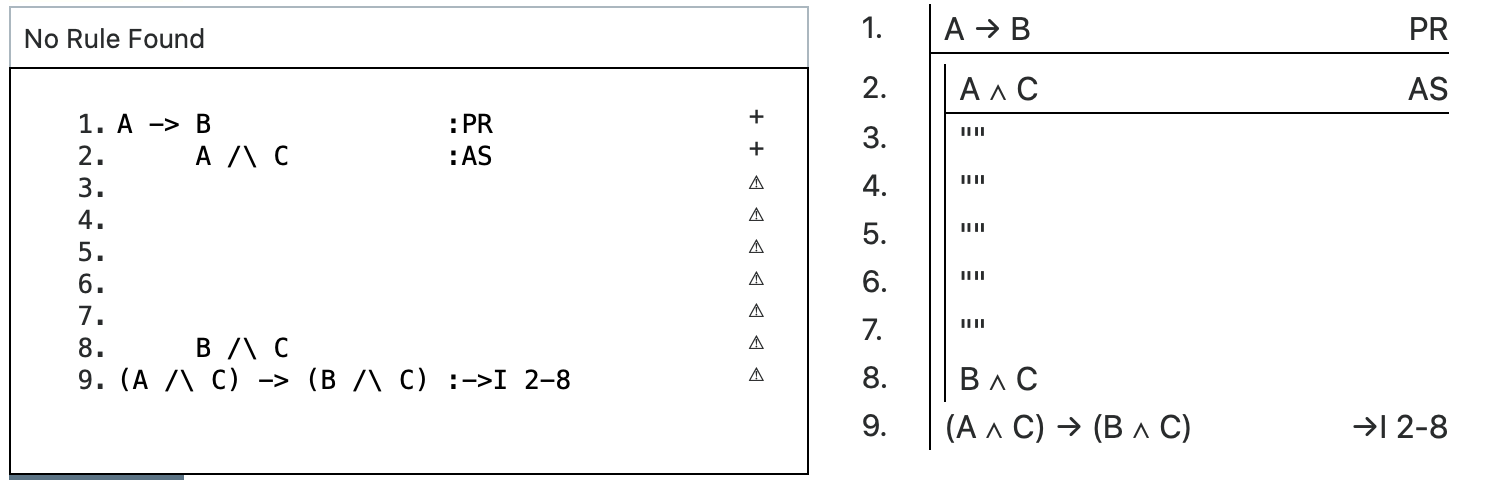
\includegraphics[width=\textwidth,height=0.75\textheight]{5_4i.png}
\caption{Setting up \(\rightarrow\)I}
\end{figure}
\end{frame}

\begin{frame}{\(A \rightarrow B \vdash (A \wedge C) \rightarrow (B \wedge C)\)}
\protect\hypertarget{a-rightarrow-b-vdash-a-wedge-c-rightarrow-b-wedge-c-2}{}
\begin{figure}
\centering
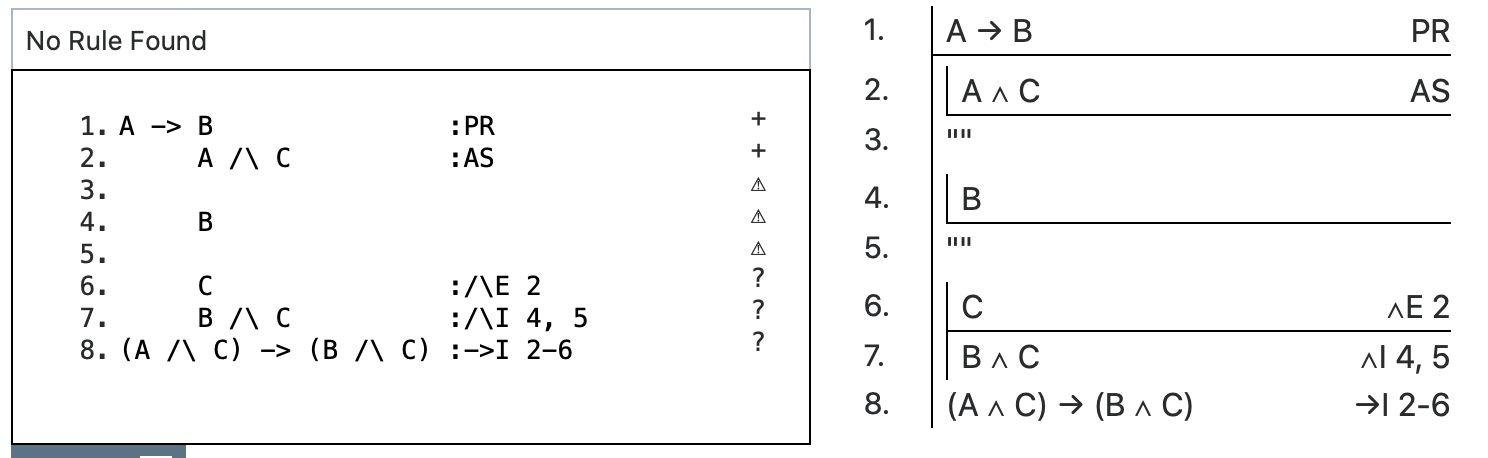
\includegraphics[width=\textwidth,height=0.75\textheight]{5_4ii.png}
\caption{Setting up \(\wedge\)I}
\end{figure}
\end{frame}

\begin{frame}{\(A \rightarrow B \vdash (A \wedge C) \rightarrow (B \wedge C)\)}
\protect\hypertarget{a-rightarrow-b-vdash-a-wedge-c-rightarrow-b-wedge-c-3}{}
\begin{figure}
\centering
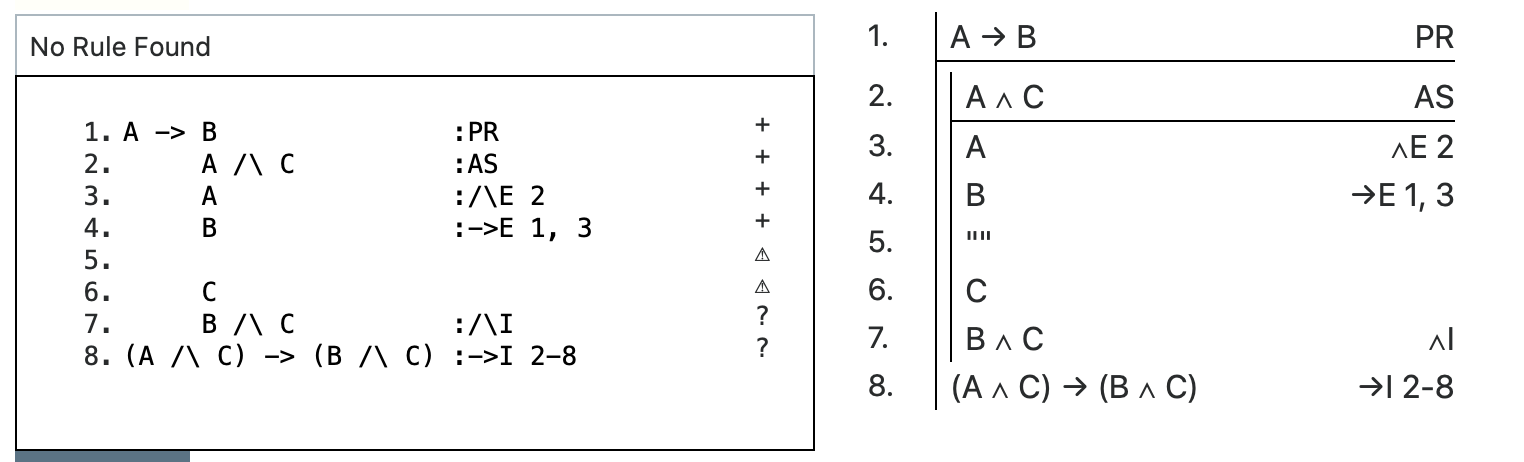
\includegraphics[width=\textwidth,height=0.75\textheight]{5_4j.png}
\caption{Getting the first conjunct}
\end{figure}
\end{frame}

\begin{frame}{\(A \rightarrow B \vdash (A \wedge C) \rightarrow (B \wedge C)\)}
\protect\hypertarget{a-rightarrow-b-vdash-a-wedge-c-rightarrow-b-wedge-c-4}{}
\begin{figure}
\centering
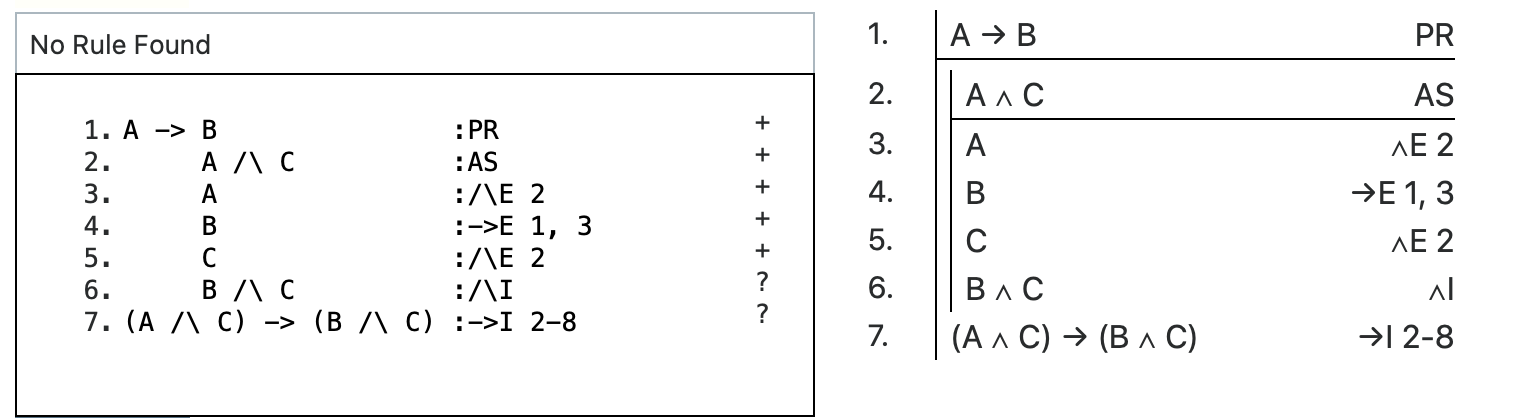
\includegraphics[width=\textwidth,height=0.75\textheight]{5_4k.png}
\caption{Getting the second conjunct}
\end{figure}
\end{frame}

\begin{frame}{\(A \rightarrow B \vdash (A \wedge C) \rightarrow (B \wedge C)\)}
\protect\hypertarget{a-rightarrow-b-vdash-a-wedge-c-rightarrow-b-wedge-c-5}{}
\begin{figure}
\centering
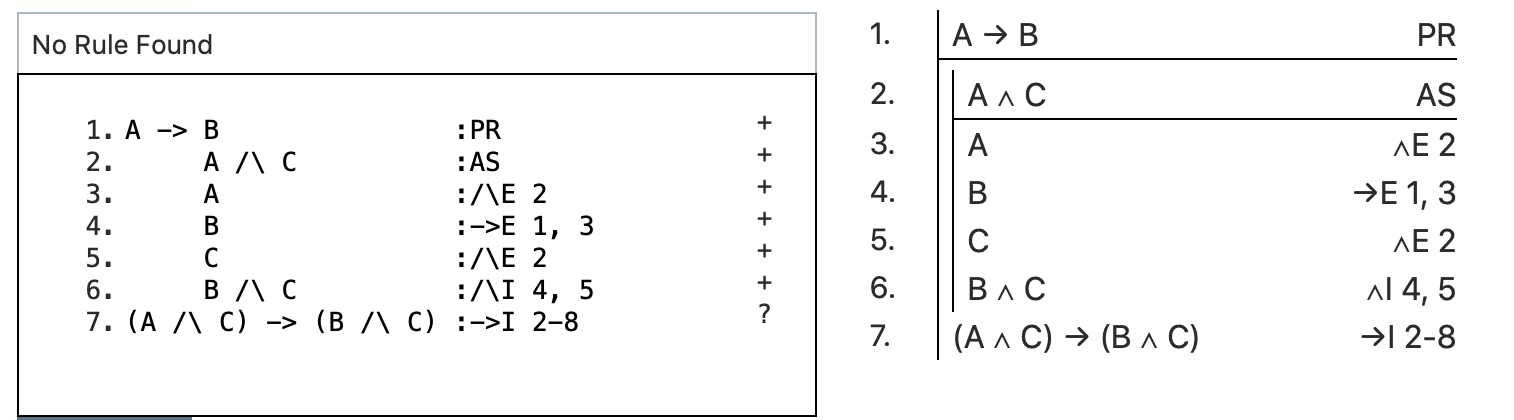
\includegraphics[width=\textwidth,height=0.75\textheight]{5_4l.png}
\caption{Line numbers for the \(\wedge\)I step}
\end{figure}
\end{frame}

\begin{frame}{\(A \rightarrow B \vdash (A \wedge C) \rightarrow (B \wedge C)\)}
\protect\hypertarget{a-rightarrow-b-vdash-a-wedge-c-rightarrow-b-wedge-c-6}{}
\begin{figure}
\centering
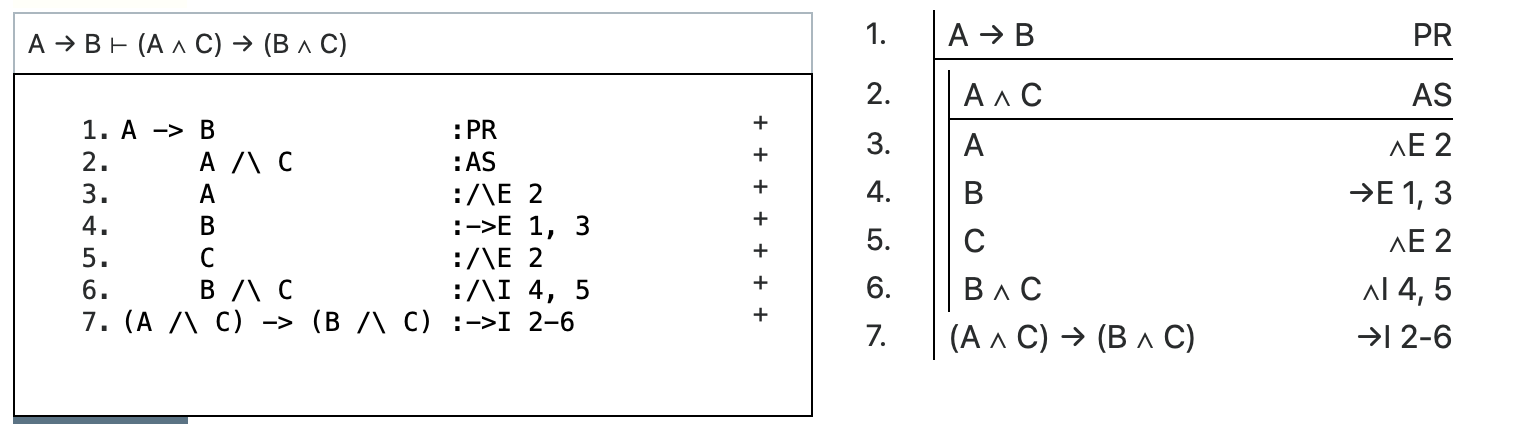
\includegraphics[width=\textwidth,height=0.75\textheight]{5_4m.png}
\caption{Line numbers for the \(\rightarrow\)I step}
\end{figure}
\end{frame}

\begin{frame}{\(A \rightarrow B, \neg B \vdash \neg A\)}
\protect\hypertarget{a-rightarrow-b-neg-b-vdash-neg-a}{}
\begin{figure}
\centering
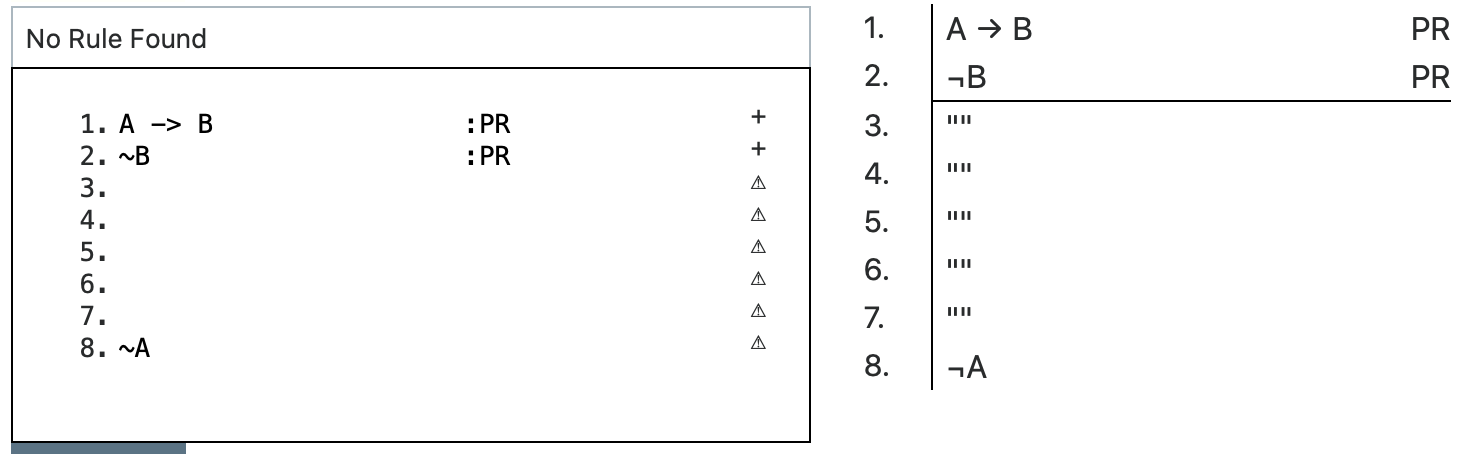
\includegraphics[width=\textwidth,height=0.75\textheight]{5_4n.png}
\caption{Premises and Conclusion}
\end{figure}
\end{frame}

\begin{frame}{\(A \rightarrow B, \neg B \vdash \neg A\)}
\protect\hypertarget{a-rightarrow-b-neg-b-vdash-neg-a-1}{}
\begin{figure}
\centering
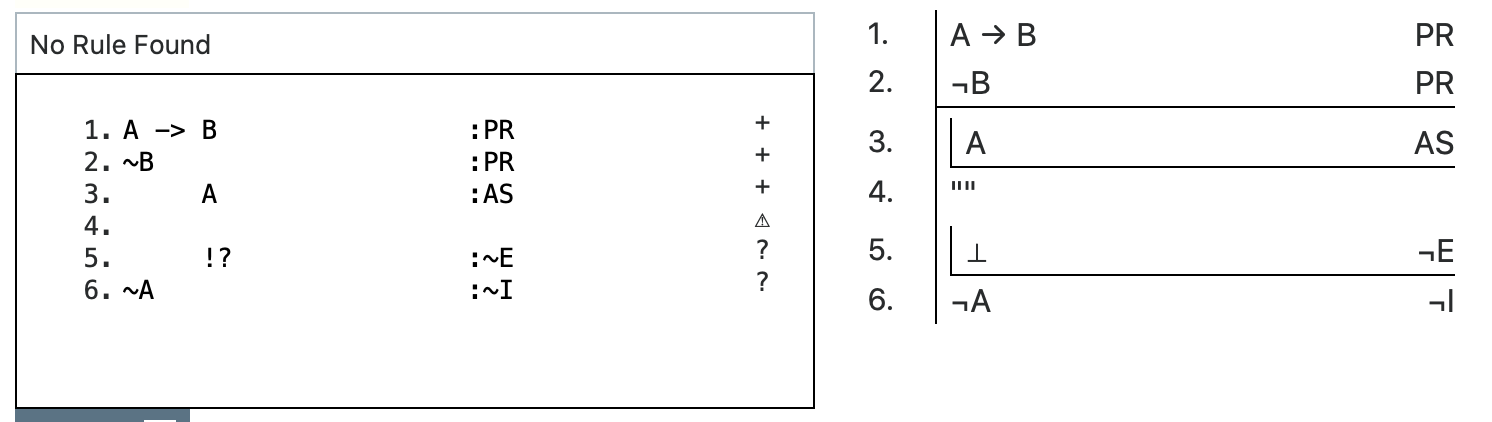
\includegraphics[width=\textwidth,height=0.75\textheight]{5_4o.png}
\caption{Setting up \(\neg\)I}
\end{figure}
\end{frame}

\begin{frame}{\(A \rightarrow B, \neg B \vdash \neg A\)}
\protect\hypertarget{a-rightarrow-b-neg-b-vdash-neg-a-2}{}
\begin{figure}
\centering
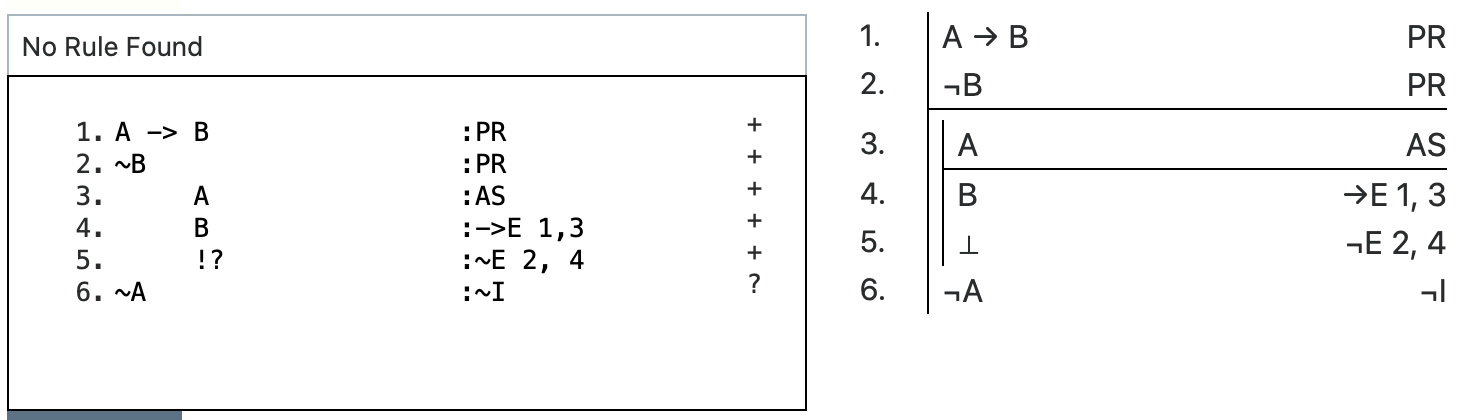
\includegraphics[width=\textwidth,height=0.75\textheight]{5_4p.png}
\caption{Getting the Contradiction}
\end{figure}
\end{frame}

\begin{frame}{\(A \rightarrow B, \neg B \vdash \neg A\)}
\protect\hypertarget{a-rightarrow-b-neg-b-vdash-neg-a-3}{}
\begin{figure}
\centering
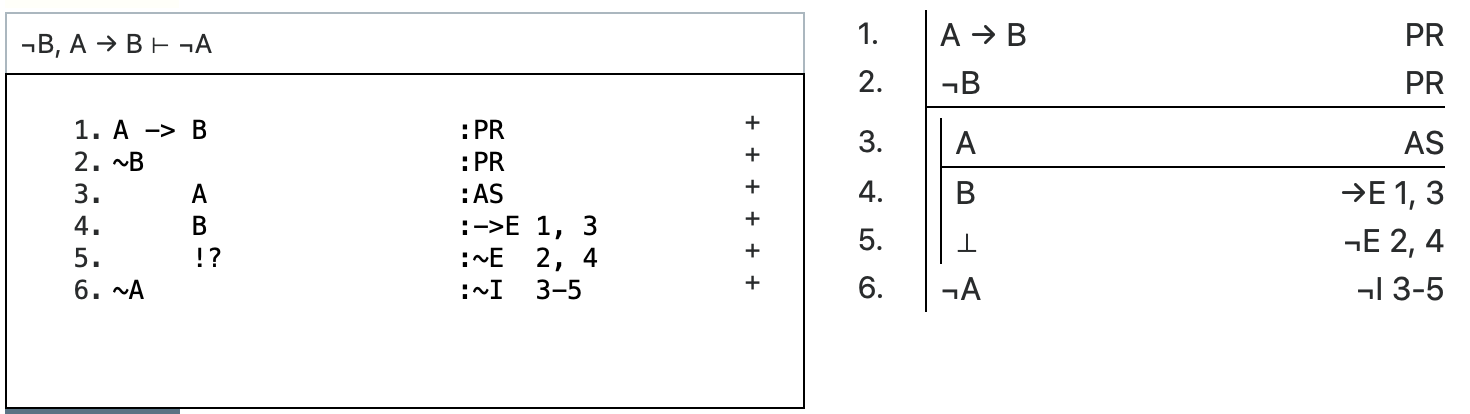
\includegraphics[width=\textwidth,height=0.75\textheight]{5_4q.png}
\caption{Finishing the Proof}
\end{figure}
\end{frame}

\begin{frame}{Working Backwards}
\protect\hypertarget{working-backwards}{}
\begin{itemize}
\tightlist
\item
  What if the conclusion is a disjunction?
\item
  Don't work backwards!
\end{itemize}
\end{frame}

\begin{frame}{For Next Time}
\protect\hypertarget{for-next-time}{}
\begin{itemize}
\tightlist
\item
  We'll look at strategies that involve going forwards.
\end{itemize}
\end{frame}

\end{document}
